\graphicspath{{content/appendices/figures}}
\chapter{Suppression Effects from Improper \texttt{Tanh} Activation}
\label{appendix:tanh_removal}

Before final evaluations could be conducted, a critical implementation flaw affecting early model performance was identified. Initially all \gls{ml} models, except \gls{convtasnet}, included a \texttt{Tanh} activation function at the output layer. This was based on the assumption that constraining the real and imaginary spectrogram outputs to the range \([-1, 1]\) would improve numerical stability during \gls{istft} reconstruction.

However, during early testing and visualization, this constraint was found to significantly suppress amplitude dynamics. The outputs became unnaturally flattened, leading to degraded waveform clarity and poor denoising metrics. \gls{snr}, \gls{pesq}, and \gls{stoi} scores in particular, even when models appeared to converge during training.

This effect is illustrated clearly in Figures~\ref{fig:suppresed_waveform} and~\ref{fig:suppresed_spectrogram}, models when trained with \texttt{Tanh} applied. The waveforms exhibit a flattened energy profile, and the spectrograms lack contrast and high-frequency content.

\begin{figure}[H]
    \centering
    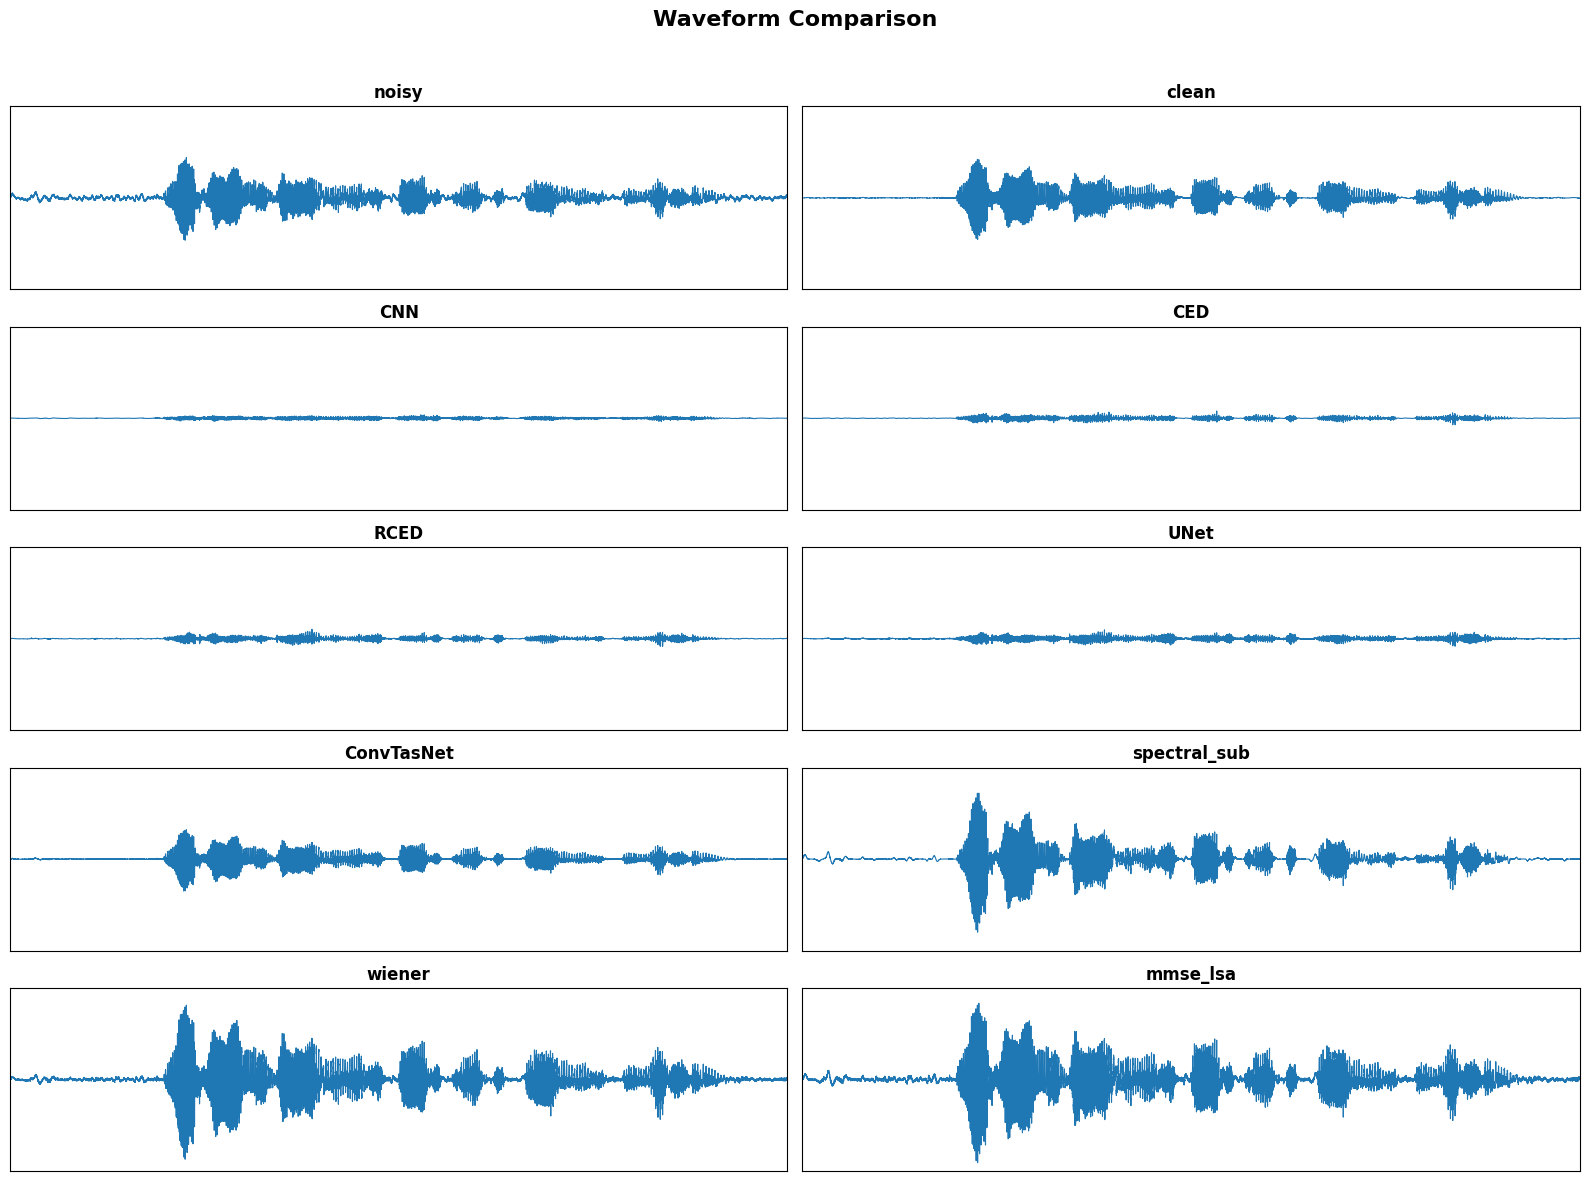
\includegraphics[width=0.9\textwidth]{suppresed_waveform.png}
    \caption{\label{fig:suppresed_waveform} Flattened waveform energy caused by \texttt{Tanh} activation. Output amplitude is artificially suppressed.}
\end{figure}

\begin{figure}[H]
    \centering
    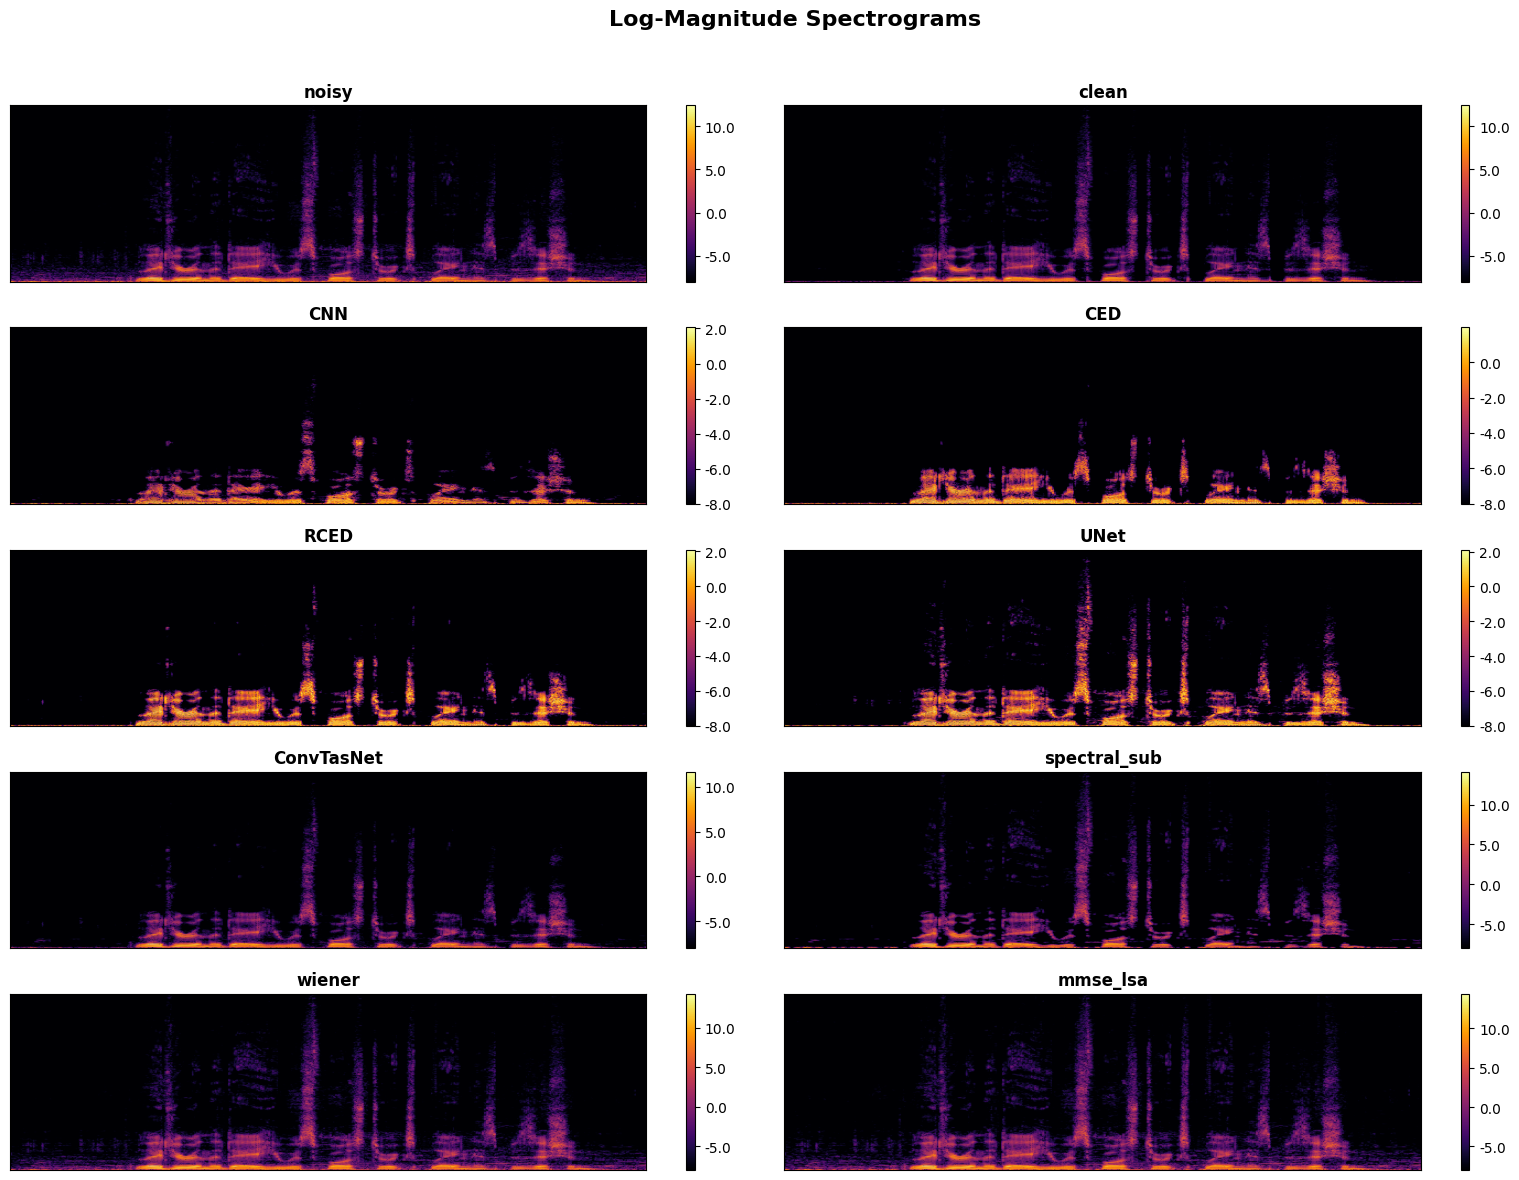
\includegraphics[width=0.9\textwidth]{suppresed_spectrogram.png}
    \caption{\label{fig:suppresed_spectrogram} Spectrograms with \texttt{Tanh} activation exhibit reduced contrast and dynamic range.}
\end{figure}

Initially, the output layer consisted of a \texttt{Tanh} activation function, followed by a bilinear interpolation step to match the output size to the input, and finally a separation of the real and imaginary components. After removing the \texttt{Tanh} activation, the output layer was simplified to include only bilinear interpolation followed by real–imaginary separation. This adjustment restored the amplitude range and natural structure in both waveform shape and spectrogram clarity, as clearly illustrated in Figures~\ref{fig:restored_waveform} and~\ref{fig:restored_spectrogram}.

\begin{figure}[H]
    \centering
    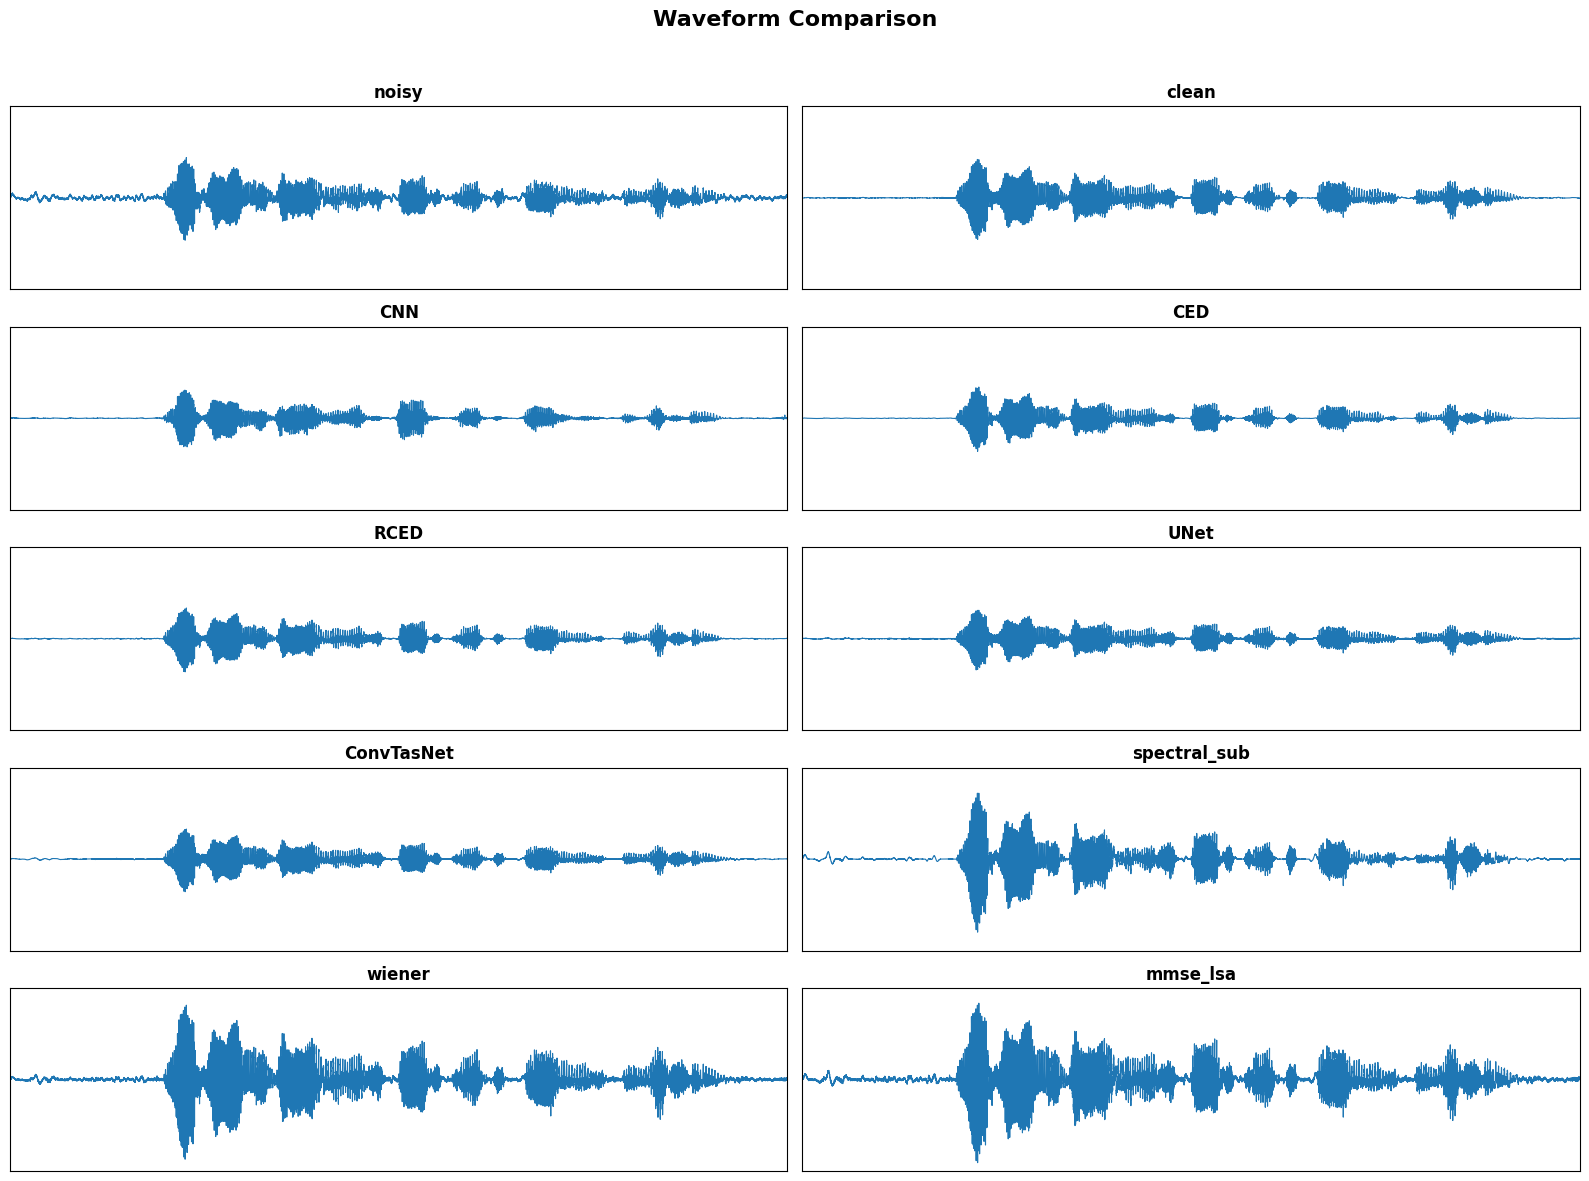
\includegraphics[width=0.9\textwidth]{fixed_waveform.png}
    \caption{\label{fig:restored_waveform} Corrected waveform comparison after removing \texttt{Tanh}. Energy and dynamics are restored.}
\end{figure}

\begin{figure}[H]
    \centering
    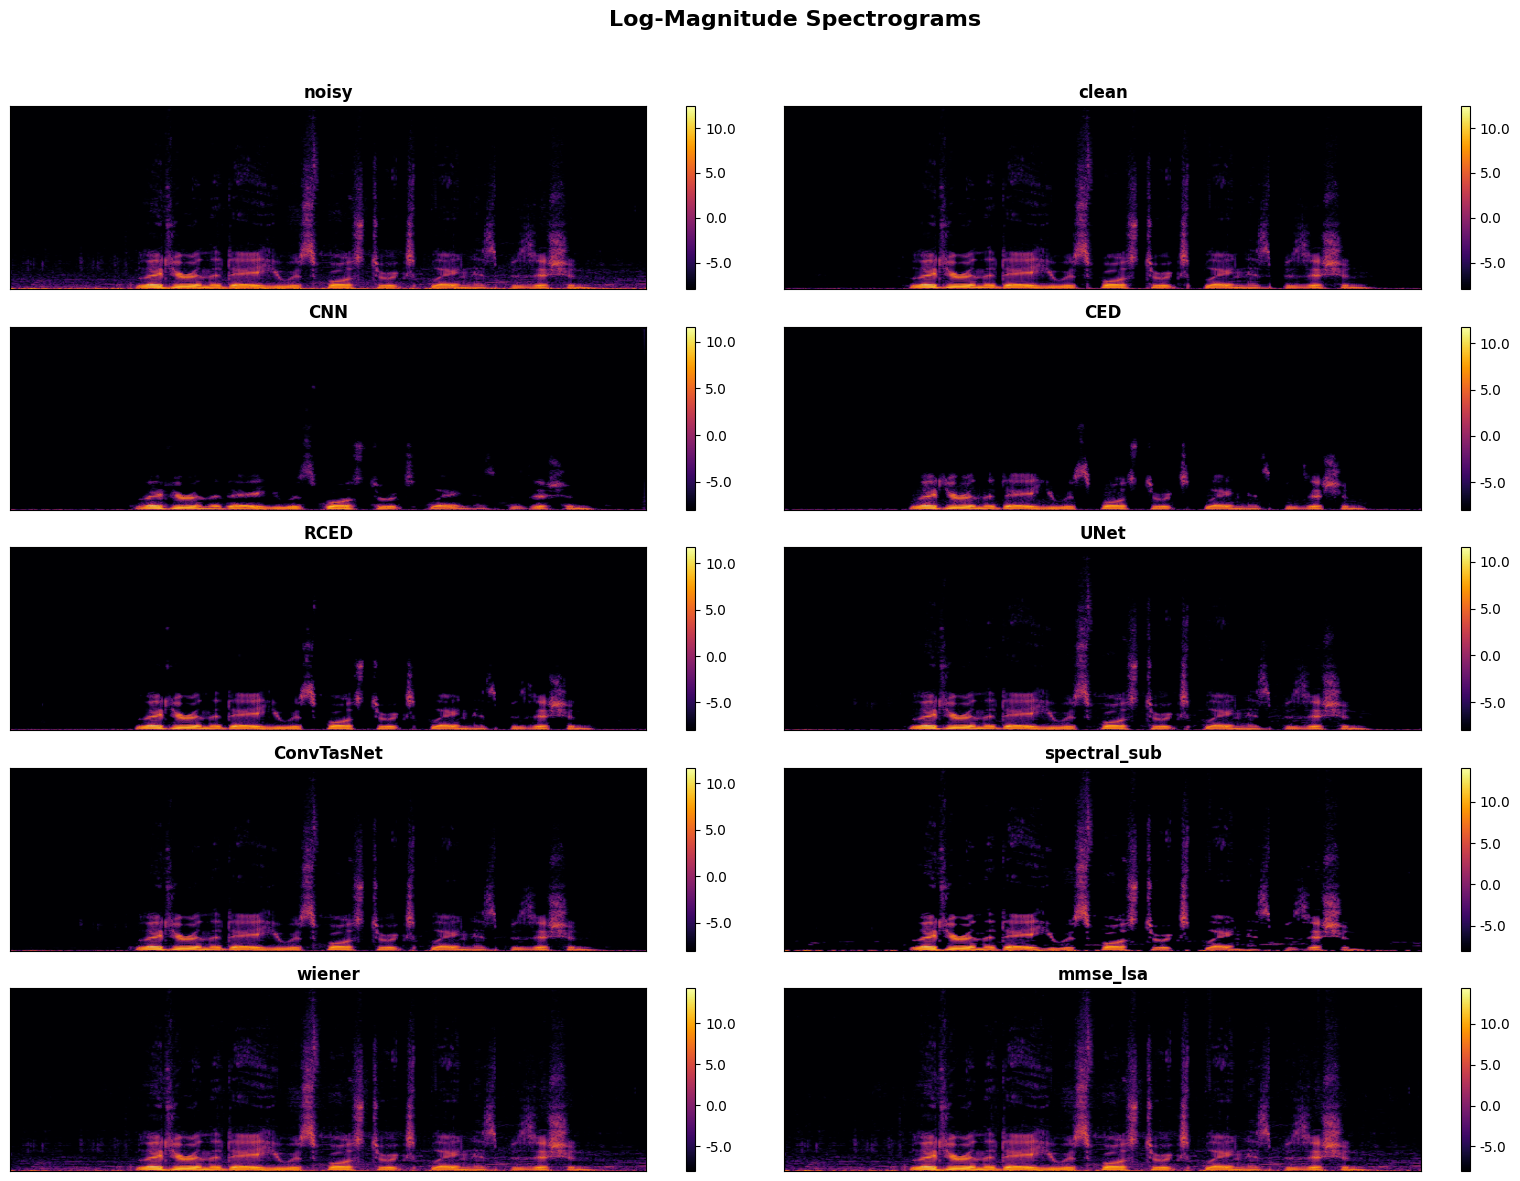
\includegraphics[width=0.9\textwidth]{fixed_spectrogram.png}
    \caption{\label{fig:restored_spectrogram} Log-magnitude spectrograms showing a restored dynamic range and greater clarity.}
\end{figure}

All final models, presented in Chapter~\ref{chp:evaluation} were retrained without the \texttt{Tanh} activation. This correction proved critical to achieving meaningful denoising results and validates the importance of properly scaled output layers in spectrogram-based models.
